\documentclass[12pt]{article}
\usepackage[T2A]{fontenc}
\usepackage[russian, english]{babel}
\usepackage[utf8x]{inputenc}
\usepackage{amsmath, amssymb}
\usepackage{graphicx}
\usepackage{physics}
\usepackage{float}
\usepackage{booktabs} 
\usepackage{amsmath}
\usepackage{systeme}
\usepackage{blindtext}
\usepackage{enumitem}
\usepackage{listings}
\usepackage[table]{xcolor}
\usepackage{mathtools}
\usepackage{hyperref}
\usepackage{tikz}
\usepackage{titlesec}
\usepackage{mathtools}
\usepackage{tcolorbox}
\usepackage{bm}
\usepackage[normalem]{ulem}
\usepackage{geometry}
\usepackage{siunitx}
\usepackage{xcolor}
\usepackage{tikzsymbols}
\usepackage{relsize}
\usepackage{pgfplots}
\usepackage[edges]{forest}
\usepackage{minted}
\usepackage{csquotes}
\usepackage{pgfplots}
\usepackage{color}
\usepackage{textcomp}
\usepackage{subcaption}
\usepackage{tikz}
\usepackage{tikz-3dplot}
\usepackage{tkz-euclide}

\makeatletter
\renewcommand\paragraph{\@startsection{paragraph}{4}{\z@}%
            {-2.5ex\@plus -1ex \@minus -.25ex}%
            {1.25ex \@plus .25ex}%
            {\normalfont\normalsize\bfseries}}
\makeatother
\setcounter{secnumdepth}{4} % how many sectioning levels to assign numbers to
\setcounter{tocdepth}{4}    % how many sectioning levels to show in ToC


\newcommand{\heart}{\ensuremath\heartsuit}
\newcommand{\butt}{\rotatebox[origin=c]{180}{\heart}}

% Redefine rotation sequence for tikz3d-plot to z-y-x
\newcommand{\tdseteulerxyz}{
  \renewcommand{\tdplotcalctransformrotmain}{%
    %perform some trig for the Euler transformation
      \tdplotsinandcos{\sinalpha}{\cosalpha}{\tdplotalpha}
    \tdplotsinandcos{\sinbeta}{\cosbeta}{\tdplotbeta}
    \tdplotsinandcos{\singamma}{\cosgamma}{\tdplotgamma}
    %
      \tdplotmult{\sasb}{\sinalpha}{\sinbeta}
    \tdplotmult{\sasg}{\sinalpha}{\singamma}
    \tdplotmult{\sasbsg}{\sasb}{\singamma}
    %
      \tdplotmult{\sacb}{\sinalpha}{\cosbeta}
    \tdplotmult{\sacg}{\sinalpha}{\cosgamma}
    \tdplotmult{\sasbcg}{\sasb}{\cosgamma}
    %
      \tdplotmult{\casb}{\cosalpha}{\sinbeta}
    \tdplotmult{\cacb}{\cosalpha}{\cosbeta}
    \tdplotmult{\cacg}{\cosalpha}{\cosgamma}
    \tdplotmult{\casg}{\cosalpha}{\singamma}
    %
      \tdplotmult{\cbsg}{\cosbeta}{\singamma}
    \tdplotmult{\cbcg}{\cosbeta}{\cosgamma}
    %
      \tdplotmult{\casbsg}{\casb}{\singamma}
    \tdplotmult{\casbcg}{\casb}{\cosgamma}
    %
      %determine rotation matrix elements for Euler transformation
      \pgfmathsetmacro{\raaeul}{\cacb}
    \pgfmathsetmacro{\rabeul}{\casbsg - \sacg}
    \pgfmathsetmacro{\raceul}{\sasg + \casbcg}
    \pgfmathsetmacro{\rbaeul}{\sacb}
    \pgfmathsetmacro{\rbbeul}{\sasbsg + \cacg}
    \pgfmathsetmacro{\rbceul}{\sasbcg - \casg}
    \pgfmathsetmacro{\rcaeul}{-\sinbeta}
    \pgfmathsetmacro{\rcbeul}{\cbsg}
    \pgfmathsetmacro{\rcceul}{\cbcg}
  }
}

% Set the plot display orientation
% Syntax: \tdplotsetdisplay{\theta_d}{\phi_d}
\tdplotsetmaincoords{60}{140}

\pgfmathsetmacro{\zRot}{10}
\pgfmathsetmacro{\yRot}{10}
\pgfmathsetmacro{\xRot}{10}

\geometry{
    a4paper,
    left=2cm,
    right=2cm,
    top=1.5cm,
    bottom=1.5cm
}
\usepackage{multicol}

\usemintedstyle{emacs}

\setminted[cpp]{ %
    linenos=true,             % Line numbers
    autogobble=true,          % Automatically remove common white space
    frame=lines,
    framesep=2mm,
    fontsize=\footnotesize,
}

\makeatletter
\newenvironment{code}
 {\RecustomVerbatimEnvironment{Verbatim}{BVerbatim}{}%
  \def\FV@BProcessLine##1{%
    \hbox{%
      \hbox to\z@{\hss\theFancyVerbLine\kern\FV@NumberSep}%
      \FancyVerbFormatLine{##1}%
    }%
  }%
  \VerbatimEnvironment
  \setbox\z@=\hbox\bgroup
  \begin{minted}{cpp}}
 {\end{minted}\egroup
  \leavevmode\vbox{\hrule\kern2mm\box\z@\kern2mm\hrule}}
\makeatother

\definecolor{mintedbackground}{rgb}{0.95,0.95,0.95}

\newmintedfile[cmakecode]{cmake}{
bgcolor=mintedbackground,
fontfamily=tt,
linenos=true,
numberblanklines=true,
numbersep=5pt,
gobble=0,
frame=leftline,
framerule=0.4pt,
framesep=2mm,
funcnamehighlighting=true,
tabsize=4,
obeytabs=false,
mathescape=false
samepage=false, %with this setting you can force the list to appear on the same page
showspaces=false,
showtabs =false,
texcl=false,
}

\definecolor{mygray}{rgb}{0.4,0.4,0.4}
\definecolor{mygreen}{rgb}{0,0.8,0.6}
\definecolor{myorange}{rgb}{1.0,0.4,0}

\lstset{
basicstyle=\footnotesize\sffamily\color{black},
commentstyle=\color{mygray},
frame=single,
numbers=left,
numbersep=5pt,
numberstyle=\tiny\color{mygray},
keywordstyle=\color{mygreen},
showspaces=false,
showstringspaces=false,
stringstyle=\color{myorange},
tabsize=2
}

\pgfmathdeclarefunction{gauss}{2}{\pgfmathparse{1/(#2*sqrt(2*pi))*exp(-((x-#1)^2)/(2*#2^2))}}

\DeclareRobustCommand{\bbone}{\text{\usefont{U}{bbold}{m}{n}1}}

\DeclareMathOperator{\EX}{\mathbb{E}}

\newcommand{\icol}[1]{% inline column vector
  \left[\begin{smallmatrix}#1\end{smallmatrix}\right]%
}


\titleclass{\subsubsubsection}{straight}[\subsection]

\newcounter{subsubsubsection}[subsubsection]
\renewcommand\thesubsubsubsection{\thesubsubsection.\arabic{subsubsubsection}}
\renewcommand\theparagraph{\thesubsubsubsection.\arabic{paragraph}} % optional; useful if paragraphs are to be numbered

% Set paragraph indent
\setlength{\parindent}{4ex}

% Set the header of the ToC as "Оглавление"
\addto\captionsenglish{
  \renewcommand{\contentsname}
    {Оглавление}
}

\titleformat{\subsubsubsection}
  {\normalfont\normalsize\bfseries}{\thesubsubsubsection}{1em}{}
\titlespacing*{\subsubsubsection}
{0pt}{3.25ex plus 1ex minus .2ex}{1.5ex plus .2ex}

\makeatletter
\renewcommand\paragraph{\@startsection{paragraph}{5}{\z@}%
  {3.25ex \@plus1ex \@minus.2ex}%
  {-1em}%
  {\normalfont\normalsize\bfseries}}
\renewcommand\subparagraph{\@startsection{subparagraph}{6}{\parindent}%
  {3.25ex \@plus1ex \@minus .2ex}%
  {-1em}%
  {\normalfont\normalsize\bfseries}}
\def\toclevel@subsubsubsection{4}
\def\toclevel@paragraph{5}
\def\toclevel@paragraph{6}
\def\l@subsubsubsection{\@dottedtocline{4}{7em}{4em}}
\def\l@paragraph{\@dottedtocline{5}{10em}{5em}}
\def\l@subparagraph{\@dottedtocline{6}{14em}{6em}}
\makeatother

\setcounter{secnumdepth}{4}
\setcounter{tocdepth}{4}

\hypersetup{
	colorlinks=true,
    linkcolor=blue,
    filecolor=magenta,      
    urlcolor=cyan,
}

\definecolor{codegreen}{rgb}{0,0.6,0}
\definecolor{codegray}{rgb}{0.5,0.5,0.5}
\definecolor{codepurple}{rgb}{0.58,0,0.82}
\definecolor{backcolour}{rgb}{0.95,0.95,0.92}

\lstdefinestyle{mystyle}{
    backgroundcolor=\color{backcolour},   
    commentstyle=\color{codegreen},
    keywordstyle=\color{magenta},
    numberstyle=\tiny\color{codegray},
    stringstyle=\color{codepurple},
    basicstyle=\ttfamily\footnotesize,
    breakatwhitespace=false,         
    breaklines=true,                 
    captionpos=b,                    
    keepspaces=true,                 
    numbers=left,                    
    numbersep=5pt,                  
    showspaces=false,                
    showstringspaces=false,
    showtabs=false,                  
    tabsize=2
}

\pagenumbering{arabic}

\begin{document}
    \begin{titlepage}
    \center % Center everything on the page
    \newcommand{\HRline}[1]{\rule{\linewidth}{#1}} % Defines a new command for the horizontal lines, change thickness here
    %----------------------------------------------------------------------------------------
    %	HEADING SECTIONS
    %----------------------------------------------------------------------------------------

    
\includegraphics[scale=1]{images/logo.jpg}\\[1cm] % Include a department/university logo - this will require the graphicx package
    \textbf{\large МИНОБРНАУКИ РОССИИ}\\[0.5cm]
    \textbf{\large федеральное государственное бюджетное образовательное учреждение}\\[0.2cm]
    \textbf{\large высшего образования}\\[0.2cm]
    \textbf{\large <<Московский государственный технологический университет}\\[0.2cm]
    \textbf{<<СТАНКИН>>}\\[0.5cm]

    \textbf{\large (ФГБОУ ВО «МГТУ «СТАНКИН»)}
    \HRline{0.02cm} \\[0.1cm]

    \begin{multicols}{2}
        \begin{flushleft}
            \textbf{\large Институт}\\
            \textbf{\large информационных}\\
            \textbf{\large систем и технологий}\\
        \end{flushleft}
        
        \columnbreak
        \begin{flushleft}
            \textbf{\large Кафедра}\\
            \textbf{\large информационных систем}\\
        \end{flushleft}

    \end{multicols}

    %----------------------------------------------------------------------------------------
    %	TITLE SECTION
    %----------------------------------------------------------------------------------------
    \textbf{\large Программирование специализированных вычислительных устройств}\\
    \textbf{\large Отчет по лабораторной работе}\\[0.5cm]


    { \Large \bfseries <<3D моделлирование посредством OpenGL для Веба>> Часть \textnumero 2}\\ % Title of your document
    \HRline{0.02cm} \\[1.5cm]
    
    %----------------------------------------------------------------------------------------
    %	AUTHOR SECTION
    %----------------------------------------------------------------------------------------

    \begin{minipage}{\textwidth}
    \begin{multicols}{2}
        \begin{flushleft}
            \large Студент группы ИДБ-19-07:\\
            \large Проверил доцент кафедры ИС:
        \end{flushleft}

        
        \columnbreak
        \begin{flushright}
            \large Касьян А.И.\\
            \large к.т.н. Волкова О.Р.
        \end{flushright}

    \end{multicols}

    \end{minipage}\\[8cm]

    % If you don't want a supervisor, uncomment the two lines below and remove the section above
    %\Large \emph{Author:}\\
    %John \textsc{Smith}\\[3cm] % Your name

    %----------------------------------------------------------------------------------------
    %	DATE SECTION
    %----------------------------------------------------------------------------------------

    {\large \today}\\[2cm] % Date, change the \today to a set date if you want to be precise


    \end{titlepage}

    \newpage

    \tableofcontents

    \newpage
    \section{Вводное слово}
    \begin{itemize}
        \item В предыдущем документе мы рассмотрели шейдеры и их обработку.
        В этом я сделаю упор на трансформациях и текстурах, в связи 
        с этим я более детально рассмотрю код самих шейдеров. 
        \item Все используемые технологии сохранились с предыдущего файла.
    \end{itemize}
    
    \section{Результат выполнения задания}
    Данную секцию я разобью на две подсекции:
    \begin{itemize}
        \item Текстурирование 
        \item Трансформация
    \end{itemize}
    \subsection{Текстурирование}
    На данный момент, пока я не имею света, текстурирование - это обычная
    отрисовка картинки, как только появится свет можно будет применять
    материалы. Оброботчик текстур я так же как и оброботчик шейдеров
    занёс в отдельный класс, вот его прототип:

    \begin{minted}{cpp}
class Texture
{
  public:
    Texture(const char *file_name, unsigned int type);
    inline unsigned int getID() const;
    void bind(const int texture_unit);
    void unbind();
    void loadFromFile(const char *file_name);
    ~Texture();

  private:
    unsigned int id;
    int width;
    int height;
    unsigned int type;
};
    \end{minted}
    Сам класс из себя ни чего не представляет. 
    В конструкторе, посредством библиотеки SOIL2 мы подгружаем картинку.
    Далее биндим текстуру и генерируем мипмэп. \texttt{\textbf{loadFromFile}} выполняет
    то же смамое, что и конструктор. \texttt{\textbf{bind}}, \texttt{\textbf{unbind}} и \texttt{\textbf{getID}}
    говорят сами за себя. Поэтому я приведу листинг только конструктора/\texttt{\textbf{loadFromFile}}:
    \begin{minted}{cpp}
Texture::Texture(const char *file_name, unsigned int type)
{
    this->type = type;

    unsigned char *image = SOIL_load_image(
                                            file_name, 
                                            &this->width,
                                            &this->height, 
                                            NULL,
                                            SOIL_LOAD_RGBA
                                          );

    // generate texture names
    glGenTextures(1, &this->id);
    glBindTexture(type, this->id);
    // Set our texture parameters
    glTexParameteri(type, GL_TEXTURE_WRAP_S, GL_REPEAT);
    glTexParameteri(type, GL_TEXTURE_WRAP_T, GL_REPEAT);
    // Set texture filtering
    glTexParameteri(type, GL_TEXTURE_MAG_FILTER, GL_LINEAR_MIPMAP_LINEAR);
    glTexParameteri(type, GL_TEXTURE_MIN_FILTER, GL_LINEAR);

    if (image)
    {
    	// specify 2d img
        glTexImage2D(type, 0, GL_RGBA, this->width, this->height, 0, GL_RGBA, GL_UNSIGNED_BYTE, image);
        glGenerateMipmap(type);
    }
    else
    {
        std::cerr << "An error has occured in the " << __FILE__ << " in line " 
                  << __LINE__ << "." << std::endl
                  << "Error occured in the: " << file_name << std::endl;
    }

    glActiveTexture(0);
    glBindTexture(type, 0);
    SOIL_free_image_data(image);
}
    \end{minted}
    Пояснять нечего.
    \subsubsection{Обработка текстур в шейдерах}
    \begin{figure}[!h]
        \begin{subfigure}{.6\textwidth}
          \begin{code}
#version 330 core
layout (location = 0) in vec3 position;
layout (location = 2) in vec2 texCoord;

out vec2 TexCoord;

uniform mat4 model;
uniform mat4 view;
uniform mat4 projection;

void main()
{
    gl_Position = projection * view * model 
                    * vec4(position, 1.0f);
    TexCoord = vec2(texCoord.x, 1.0 - texCoord.y);
}
          \end{code}
          \caption{vertex shader}
          \label{fig:sfig1}
        \end{subfigure}%
        \begin{subfigure}{.6\textwidth}
          \begin{code}
#version 330 core
in vec2 TexCoord;

out vec4 color;

uniform sampler2D ourTexture1;






void main()
{
    color = texture(ourTexture1, TexCoord);
}
          \end{code}
          \caption{fragment shader}
          \label{fig:sfig2}
        \end{subfigure}
    \end{figure}
    \begin{enumerate}
        \item \textbf{vertex shader} - Фрагмент шейдер будет принимать
        координату текстуры \texttt{TexCoord}, устанавливаем её как out.
        Считаем эту координату.
        \item \textbf{fragment shader} - Во фрагмент шейдере, нам так же требуется
        получить доступ к объекту текстуры. В GLSL есть buid-in тип данных, предназначеных
        для текстур (\textbf{\texttt{sampler*D}}, где * $\in [1-3]$), поэтому добавляем 
        глобальную текстурную переменную. Чтобы выбрать цвет текстуры, мы используем встроенную 
        функцию \texttt{texture}, которая принимает в качестве первого аргумента текстуру, 
        а в качестве второго аргумента - соответствующие координаты текстуры. Затем функция \texttt{texture} 
        выбирает соответствующее значение цвета, используя параметры текстуры, которые мы установили ранее.
        Результатом этого фрагментного шейдера является (отфильтрованный) цвет текстуры в (интерполированной) 
        координате текстуры.
    \end{enumerate}
    \subsubsection{Использование текстур}
    \begin{minted}{cpp}
int main()
{
    ...
    // the type is GL_TEXTURE_2D
    Texture texture("assets/images/image1.jpg", GL_TEXTURE_2D);
#ifdef __EMSCRIPTEN__
    std::function<void()> mainLoop = [&]() {
#else
    while (!glfwWindowShouldClose(window))
    {
#endif
        ...

        // Bind Textures using texture units
        texture.bind(0);
        ourShader.set1i(0, "ourTexture1");
        
        ...

#ifdef __EMSCRIPTEN__
    };
    emscripten_set_main_loop_arg(dispatch_main, &mainLoop, 0, 1);
#else
    }
#endif
...
}
    \end{minted}
    \subsubsection{Результат работы текстурирования}
    \begin{figure}[!h]
        \begin{subfigure}{.5\textwidth}
          \centering
          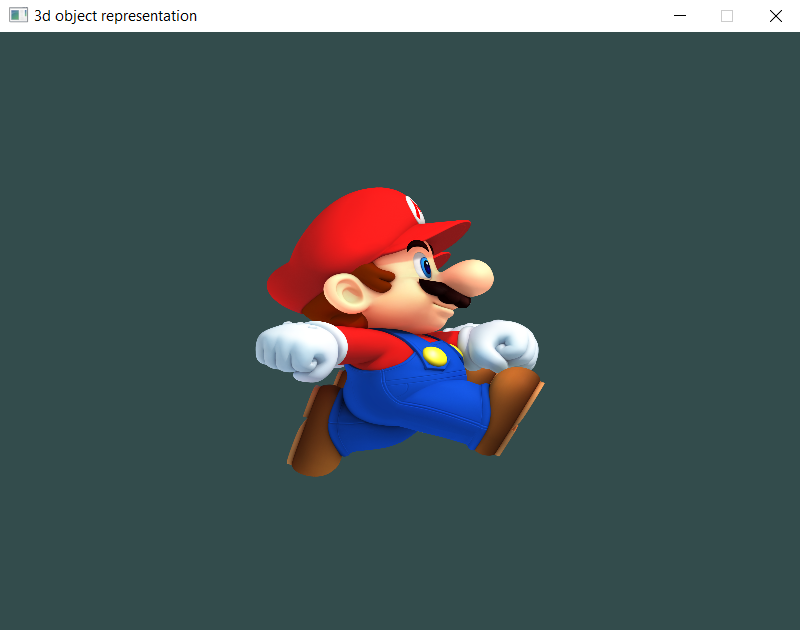
\includegraphics[width=.95\linewidth]{images/shaders_result.png}
          \caption{front}
          \label{fig:sfig3}
        \end{subfigure}%
        \begin{subfigure}{.5\textwidth}
          \centering
          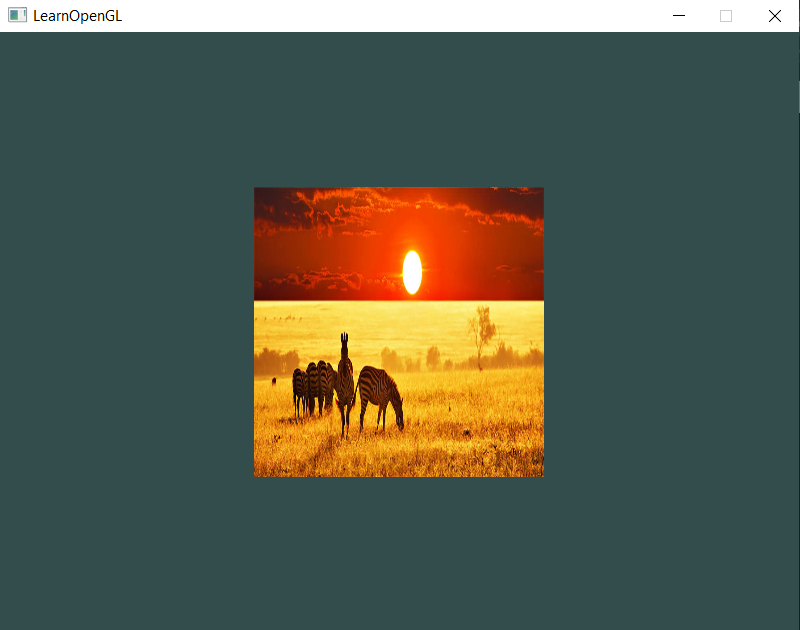
\includegraphics[width=.95\linewidth]{images/texture_res.png}
          \caption{rotation}
          \label{fig:sfig4}
        \end{subfigure}
    \end{figure}
    \subsection{Трансформация}
    На данный момент я закончил камеру, фактически трансформация хорошо описана
    камерой. Однако в дальнейшем я хочу добавить возможность вращения объекта вокруг
    нулевой точки.
    \noindent
    Прототип класса камеры выглядит так:
    \begin{minted}{cpp}
// Defines several possible options for camera movement. Used as abstraction to stay away from window-system specific
// input methods
enum Camera_Movement
{
    FORWARD,
    BACKWARD,
    LEFT,
    RIGHT
};

// Default camera values
const float YAW = -90.0f;
const float PITCH = 0.0f;
const float SPEED = 6.0f;
const float SENSITIVTY = 0.15f;
const float ZOOM = 45.0f;

class Camera
{
  public:
    Camera(glm::vec3 position = glm::vec3(0.0f, 0.0f, 0.0f), glm::vec3 up = glm::vec3(0.0f, 1.0f, 0.0f),
           float yaw = YAW, float pitch = PITCH);
    Camera(float pos_x, float pos_y, float pos_z, float up_x, float up_y, float up_z, float yaw, float pitch);
    // Returns the view matrix calculated using Eular Angles and the LookAt Matrix
    glm::mat4 GetViewMatrix();
    // Processes input received from any keyboard-like input system. 
    // Accepts input parameter in the form of camera
    void ProcessKeyboard(Camera_Movement direction, float delta_time);
    // Expects the offset value in both the x and y direction.
    void ProcessMouseMovement(float x_offset, float y_offset, unsigned char constrain_pitch = true);
    // Only requires input on the vertical wheel-axis
    void ProcessMouseScroll(float y_offset);
    float GetZoom();

  private:
    // Camera Attributes
    glm::vec3 position;
    glm::vec3 front;
    glm::vec3 up;
    glm::vec3 right;
    glm::vec3 world_up;

    // Eular Angles
    float yaw;
    float pitch;
    float roll;

    // Camera options
    float movement_speed;
    float mouse_sensitivity;
    float zoom;

    // Calculates the front vector from the Camera's (updated) Eular Angles
    void updateCameraVectors();
};
    \end{minted}
    \begin{minted}{cpp}
void Camera::updateCameraVectors()
{
    // Calculate the new Front vector
    glm::vec3 front;
    front.x = cos(glm::radians(this->yaw)) * cos(glm::radians(this->pitch));
    front.y = sin(glm::radians(this->pitch));
    front.z = sin(glm::radians(this->yaw)) * cos(glm::radians(this->pitch));
    this->front = glm::normalize(front);
    // Also re-calculate the Right and Up vector
    this->right = glm::normalize(
        glm::cross(this->front, this->world_up)); 
        // Normalize the vectors, because their length gets closer to 0 the
        // more you look up or down which results in slower movement.
    this->up = glm::normalize(glm::cross(this->right, this->front));
}
void Camera::ProcessKeyboard(Camera_Movement direction, float delta_time)
{
    float velocity = this->movement_speed * delta_time;
    switch (direction)
    {
    case FORWARD: this->position += this->front * velocity; break;
    case BACKWARD: this->position -= this->front * velocity; break;
    case LEFT: this->position -= this->right * velocity; break;
    case RIGHT: this->position += this->right * velocity; break;
    default: break;
    }
}

void Camera::ProcessMouseMovement(float x_offset, float y_offset, unsigned char constrain_pitch)
{
    x_offset *= this->mouse_sensitivity;
    y_offset *= this->mouse_sensitivity;

    this->yaw += x_offset;
    this->pitch += y_offset;

    // Make sure that when pitch is out of bounds, screen doesn't get flipped
    if (constrain_pitch)
    {
        if (this->pitch > 89.0f) { this->pitch = 89.0f; }

        if (this->pitch < -89.0f) { this->pitch = -89.0f; }
    }

    // Update Front, Right and Up Vectors using the updated Eular angles
    this->updateCameraVectors();
}

void Camera::ProcessMouseScroll(float y_offset)
{
    if (this->zoom >= 1.0f && this->zoom <= 45.0f) { this->zoom -= y_offset; }

    if (this->zoom <= 1.0f) { this->zoom = 1.0f; }

    if (this->zoom >= 45.0f) { this->zoom = 45.0f; }
}
    \end{minted}
    Так же оставляю без пояснений - коментарии всё покрывают.
    А вот сейчас самое интересное, я поясню - я не программист,
    я математик (аналитик) мне не интересен код, мне интересна логика,
    поэтому я немного разберу логику трансформаций.

    \subsubsection{Математика \Large \heart}

    \subsubsubsection{Камера: осмотр}

    Знакомтесь, \href{https://en.wikipedia.org/wiki/Euler_angles}{углы Эйлера}:

    \begin{tikzpicture}[scale=5,tdplot_main_coords]

        % Set origin of main (body) coordinate system
        \coordinate (O) at (0,0,0);
        
        % Draw main coordinate system
        \draw[red, ,->] (0,0,0) -- (1,0,0) node[anchor=north east]{$x_{\mathcal{I}}$};
        \draw[red, ,->] (0,0,0) -- (0,1,0) node[anchor=north west]{$y_{\mathcal{I}}$};
        \draw[red, ,->] (0,0,0) -- (0,0,1) node[anchor=south]{$z_{\mathcal{I}}$};
        
        % Rotate to final frame
        \tdplotsetrotatedcoords{\zRot}{\yRot}{\xRot}
        \draw[thick,tdplot_rotated_coords,->, cyan] (0,0,0) -- (1,0,0) node[anchor=west]{$x_{\mathcal{B}}$};
        \draw[thick,tdplot_rotated_coords,->, cyan] (0,0,0) -- (0,1,0) node[anchor=west]{$y_{\mathcal{B}}$};
        \draw[thick,tdplot_rotated_coords,->, cyan] (0,0,0) -- (0,0,1) node[anchor=south]{$z_{\mathcal{B}}$};
        
        %Draws circle representing the rotated planes. Each of these should be "pointed" by two arrows.
        \tdplotdrawarc[dashed,tdplot_rotated_coords,->,color=black]{(0,0,0)}{1}{0}{350}{anchor=south west,color=black}{$x-y$}
        \tdplotsetrotatedthetaplanecoords{0}
        \tdplotdrawarc[dashed,tdplot_rotated_coords,->,color=blue]{(0,0,0)}{1}{0}{350}{anchor=south west,color=blue}{$x-z$}
        \tdplotsetrotatedthetaplanecoords{90}
        \tdplotdrawarc[dashed,tdplot_rotated_coords,->,color=red]{(0,0,0)}{1}{0}{350}{anchor=south west,color=red}{$y-z$}
    \end{tikzpicture}

    \noindent
    Красиво, не правда ли. Углы Эйлера - это три угла для описания ориентации "твердого" тела относительно фиксированной системы координат.
    У этих углов есть названия:
    \begin{itemize}
        \item \textbf{pitch} - угол, отвечающий за вращение вокруг оси абсцисс (оси х)
        \item \textbf{yaw} - угол, отвечающий за вращение вокруг оси ординат (оси y)
        \item \textbf{roll} - угол, отвечающий за вращение вокруг оси аппликат (оси z)
    \end{itemize}
    \noindent
    По данной картинке всё интуитивно понятно:

    
\includegraphics[width=\linewidth]{images/camera_pitch_yaw_roll.png}

    \noindent
    Каждый угол репрезентуется одним значением. Скомбинировав эти углы 
    мы получим ротацию любого вектора в 3d пространстве.\\[0.5cm]
    \noindent
    Так как мы работаем с осмотром, посредством камеры - базовая логика углов Эйлера
    сохраняется, однако для нашей системы камеры roll-угол отпадает, за ненадобностью.
    Имея pitch и yaw значения мы можем конвертировать их в 3d вектор, который собой представляет
    Эвклидов вектор (или просто вектор). 
    Теперь определимся с двумя аксиомами (в нашем случае пусть будут аксиомы):

    \begin{multicols}{2}
      \begin{tikzpicture}[thick]
          \coordinate (O) at (0,0);
          \coordinate (A) at (4,0);
          \coordinate (B) at (0,2);
          \draw (O)--(A)--(B)--cycle;
          
          \tkzLabelSegment[below=2pt](O,A){\textit{x}}
          \tkzLabelSegment[left=2pt](O,B){\textit{y}}
          \tkzLabelSegment[above right=2pt](A,B){\textit{гипотенуза=1}}
         
          \tkzMarkAngle[fill= orange,size=0.8cm,%
          opacity=.4](B,A,O)
          \tkzLabelAngle[pos = 0.6](B,A,O){$\theta$}
        \end{tikzpicture}
        \vfill
        \columnbreak
        \begin{enumerate}
          \item {\Large $\cos(\theta) = \frac{x}{\text{гипотенуза}}$}
          \item {\Large $\sin(\theta) = \frac{y}{\text{гипотенуза}}$}
      \end{enumerate}
    \end{multicols}
    \noindent
    Если взять гипотенузу за 1, тогда мы получим $\cos(\theta) = x$ и $\sin(\theta) = y$.
    \begin{figure}[!h]
      \begin{subfigure}{.5\textwidth}
        \centering
        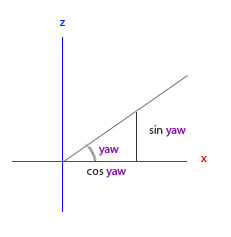
\includegraphics[width=.8\linewidth]{images/camera_yaw_coord.png}
        \caption{yaw angle}
        \label{fig:sfig5}
      \end{subfigure}%
      \begin{subfigure}{.5\textwidth}
        \centering
        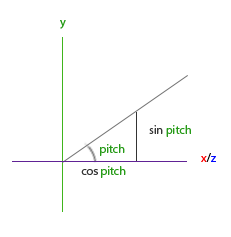
\includegraphics[width=.8\linewidth]{images/camera_pitch_coord.png}
        \caption{pitch angle}
        \label{fig:sfig6}
      \end{subfigure}
  \end{figure}

  \noindent
  Давайте представим, что yaw - это угол, идущий против часовой стрелки, начиная с оси абсцисс.
  Тогда, длина стороны по ОХ равна $cos(\text{yaw})$, длина стороны по OZ равна $sin(\text{yaw})$.
  И так мы разобрались с ккординатой в 3d пространстве, относительно оси OX.
  Теперь перейдём к оси OY, и если представить, что мы "смотрим" на OY 
  с плоскости XZ, тогда pitch строит схожий треугольник, где 
  длина стороны по OX = $cos(\text{pitch})$, длина стороны по OZ = $cos(\text{pitch})$ и
  по OY = $sin(\text{pitch})$.
  \\[0.5cm]
  \noindent
  Всё описанное выше расматривалось относительно какой-то оси.
  Но т.к. камера - объект, расположенный относительно какой-то
  точки, а не оси, то объединим всё в одно. Т.к. длины по OX и по
  OZ обе равны $cos(\text{pitch})$, однако в это же аремя $\norm{X}$ = $cos(\text{yaw})$,
  а $\norm{Z} = sin(\text{yaw})$. Тем самым, мы получили финальный вектор, транслированный
  из двух углов Эйлера.
  $$
  direction = \begin{cases} x = cos(\text{pitch}) \times cos(\text{yaw})\\ y = sin(\text{pitch}) \\  z = cos(\text{pitch}) \times sin(\text{yaw}) \end{cases}
  $$ 
  \subsubsubsection{Камера: движение}
  Ни чего интересного, просто берём позицию камеры и прибавляем к ней определённый
  вектор, помноженный на скаляр скорости. Даже замарачиваться и отрисовывать что-то не хочу.
  \subsubsubsection{Модель: вращение}
  Чуть по-позже я добавлю вращение модели.
  Выполняется посредством всё тех же углов Эйлера, только матрицы немного поменялись:

  $$
  {\displaystyle {\begin{aligned}{\begin{bmatrix}x\\y\\z\\\end{bmatrix}}&=R_{z}(\psi )R_{y}(\theta )R_{x}(\phi ){\begin{bmatrix}X\\Y\\Z\\\end{bmatrix}}\\&={\begin{bmatrix}\cos \psi &-\sin \psi &0\\\sin \psi &\cos \psi &0\\0&0&1\\\end{bmatrix}}{\begin{bmatrix}\cos \theta &0&\sin \theta \\0&1&0\\-\sin \theta &0&\cos \theta \\\end{bmatrix}}{\begin{bmatrix}1&0&0\\0&\cos \phi &-\sin \phi \\0&\sin \phi &\cos \phi \\\end{bmatrix}}{\begin{bmatrix}X\\Y\\Z\\\end{bmatrix}}\\&={\begin{bmatrix}\cos \theta \cos \psi &-\cos \phi \sin \psi +\sin \phi \sin \theta \cos \psi &\sin \phi \sin \psi +\cos \phi \sin \theta \cos \psi \\\cos \theta \sin \psi &\cos \phi \cos \psi +\sin \phi \sin \theta \sin \psi &-\sin \phi \cos \psi +\cos \phi \sin \theta \sin \psi \\-\sin \theta &\sin \phi \cos \theta &\cos \phi \cos \theta \\\end{bmatrix}}{\begin{bmatrix}X\\Y\\Z\\\end{bmatrix}}\\\end{aligned}}}
  $$
  \subsubsection{Трансформация в OpenGL}
  Кратко, как всё описанное выше работает в OpenGL:

  
\includegraphics[width=\linewidth]{images/c4_transformation.png}
  \begin{enumerate}
    \item \textbf{Model matrix} - Преобразует позицию модели в позицию в мире. Это положение зависит от положения, масштаба и поворота отрисованной модели.
    \item \textbf{View matrix} - Если в реальном мире мы двигаем камерой вокруг мира, то в OpenGL мир двигается вокруг камеры
    камера установленна на нулевой точке, с -Z направлением, т.е. если вы хотите поднять камеру - вы опускаете мир. 
    \item \textbf{Projection matrix} - после трансформации мира, выполняется проецирование (отдаляем камеру - объект уменьшается).
    У матрицы проекции есть своя фишка, её нужно нормализовать. После того как вы премените матрицу проекции
    - вы получите некоторые координаты (clip coordinates), однако знаете момент, когда вы отдаляете объект, а он растягивается.
    Это связано с FOV, чем больше угол FOV - тем больше точек в себя включает сцена.
    
    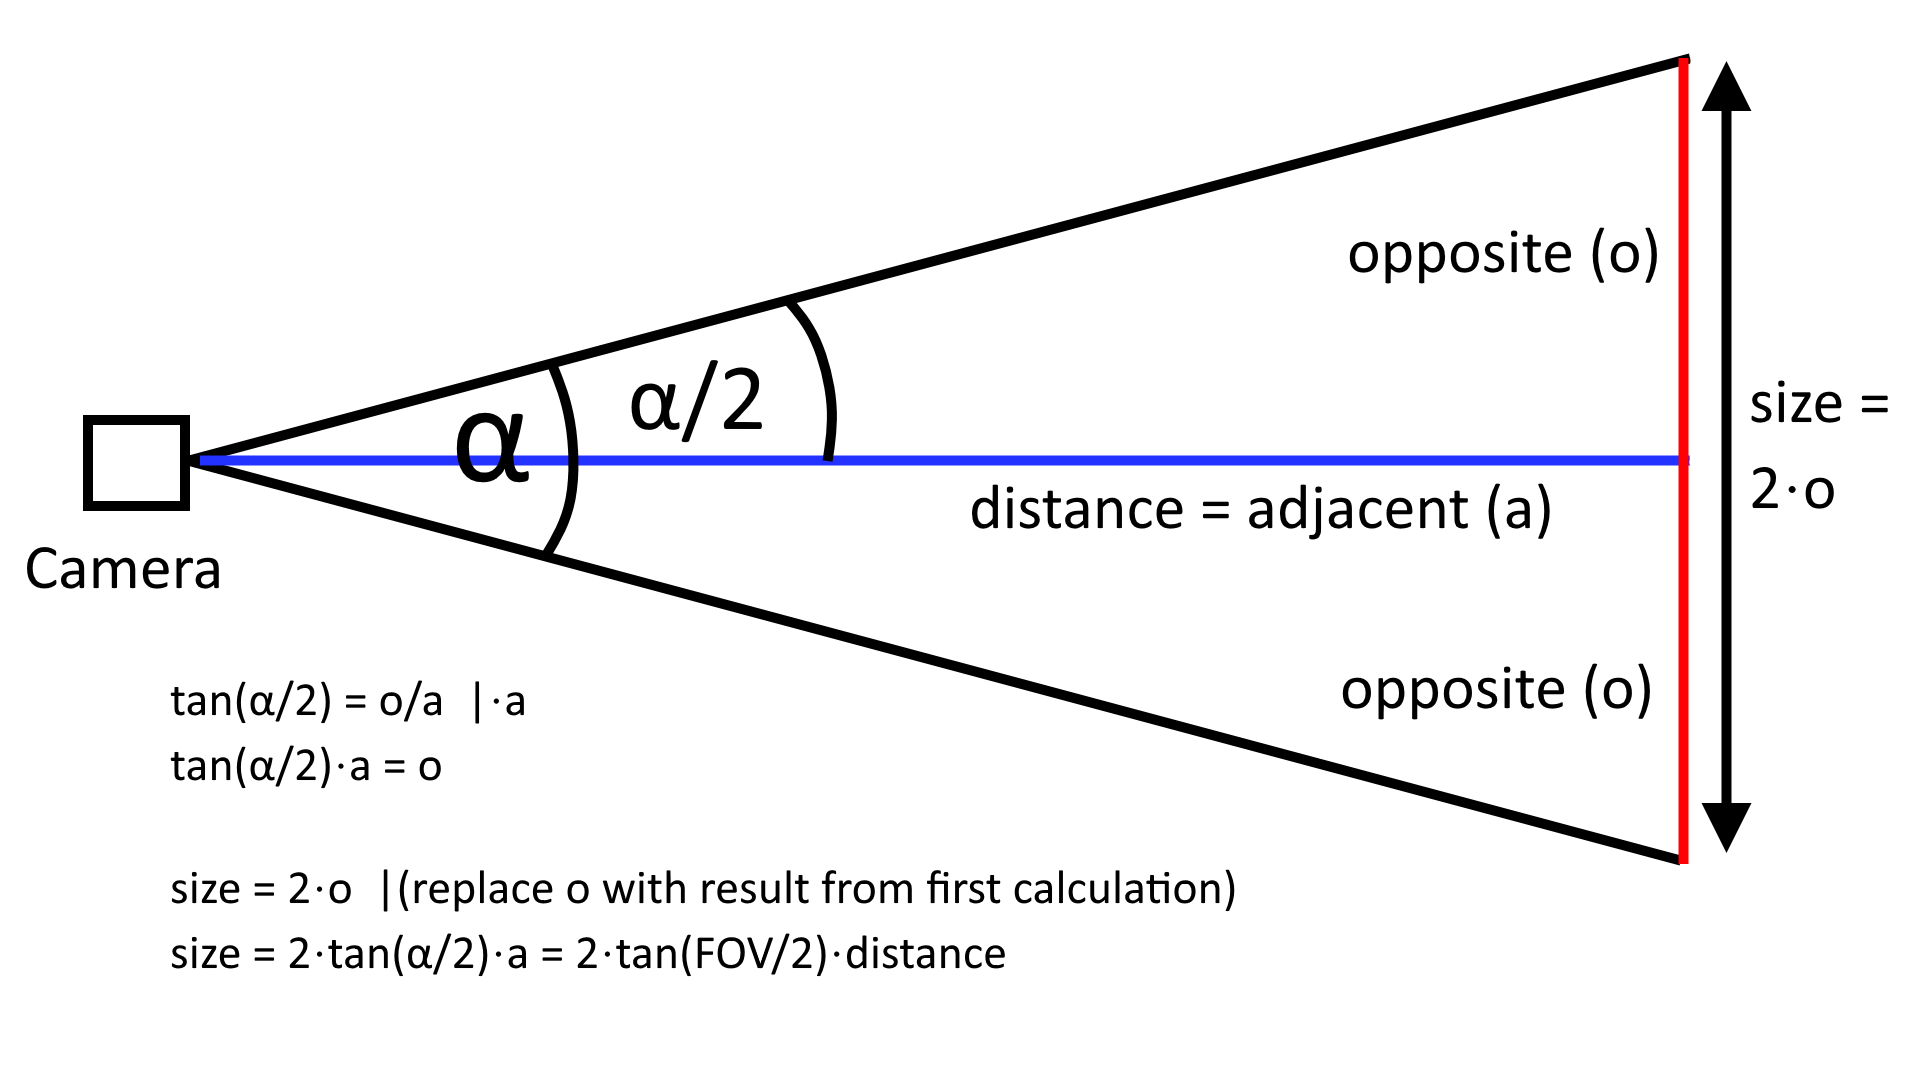
\includegraphics[width=\linewidth]{images/fov.png}
    Исходя из FOV и дистанции мы расчитываем размер объекта.
    Однако, конечный результат будет лежать в отрезке $[-1;1]$.
    И только потом подгоняем под размер сцены.
    А теперь вспомноим, что мы получили координаты в ненормализованной
    форме, а следовательно их нужно нормализовать.
    $$
      v_{\text{normalized}} = \begin{pmatrix}
        x_{clip}/w_{clip} \\
        y_{clip}/w_{clip} \\
        z_{clip}/w_{clip} \\
      \end{pmatrix}
    $$
    $w$ - показатель на сколько далеко объект находится от камеры (дистанция).
  \end{enumerate}
  \noindent
  Далее, чтобы нормально всё отобразить - мы объединяем все три матрицы в одну:
  $$
    v' = M_{\text{proj}} * M_{\text{view}} * M_{\text{model}} * v
  $$
  Вообщем-то данную операцию мы выполняем в вертекс шейдере.
  \begin{minted}{cpp}
    gl_Position = projection * view * model * vec4(position, 1.0f);
  \end{minted}
  
  \subsubsection{Использование камеры и трансформаций}

  \begin{minted}{cpp}
const GLuint WIDTH = 800, HEIGHT = 600;
int SCREEN_WIDTH, SCREEN_HEIGHT;
// Function prototypes
void KeyCallback(GLFWwindow *window, int key, int scancode, int action, int mode);
void ScrollCallback(GLFWwindow *window, double xOffset, double);
void MouseCallback(GLFWwindow *window, double xPos, double yPos);
void DoMovement();
Camera camera(glm::vec3(0.0f, 0.0f, 3.0f));
GLfloat lastX = WIDTH / 2.0;
GLfloat lastY = HEIGHT / 2.0;
bool keys[1024];
bool firstMouse = true;
GLfloat deltaTime = 0.0f;
GLfloat lastFrame = 0.0f;
int main()
{
 ...
    Texture texture("assets/images/image1.jpg", GL_TEXTURE_2D);
#ifdef __EMSCRIPTEN__
    std::function<void()> mainLoop = [&]() {
#else
    while (!glfwWindowShouldClose(window))
    {
#endif
...
        glm::mat4 projection(1);
        projection = glm::perspective(glm::radians(camera.GetZoom()), 
                    (GLfloat)SCREEN_WIDTH / (GLfloat)SCREEN_HEIGHT, 0.1f, 1000.0f);
        // Create camera transformation
        glm::mat4 view(1);
        view = camera.GetViewMatrix();
        // Pass the matrices to the shader
        ourShader.setMat4fv(view, "view");
        ourShader.setMat4fv(projection, "projection");
        glBindVertexArray(VAO);
        for (GLuint i = 0; i < 10; i++)
        {
            // Calculate the model matrix for each object and pass it to shader before drawing
            glm::mat4 model(1);
            model = glm::translate(model, cubePositions[i]);
            GLfloat angle = 20.0f * i;
            model = glm::rotate(model, angle, glm::vec3(1.0f, 0.3f, 0.5f));
            ourShader.setMat4fv(model, "model");
            ourShader.Use();
            glDrawArrays(GL_TRIANGLES, 0, 36);
        }
...
#ifdef __EMSCRIPTEN__
    };
    emscripten_set_main_loop_arg(dispatch_main, &mainLoop, 0, 1);
#else
    }
#endif
...
}
// Moves/alters the camera positions based on user input
void DoMovement()
{
    // Camera controls
    if (keys[GLFW_KEY_W] || keys[GLFW_KEY_UP]) { camera.ProcessKeyboard(FORWARD, deltaTime); }
    if (keys[GLFW_KEY_S] || keys[GLFW_KEY_DOWN]) { camera.ProcessKeyboard(BACKWARD, deltaTime); }
    if (keys[GLFW_KEY_A] || keys[GLFW_KEY_LEFT]) { camera.ProcessKeyboard(LEFT, deltaTime); }
    if (keys[GLFW_KEY_D] || keys[GLFW_KEY_RIGHT]) { camera.ProcessKeyboard(RIGHT, deltaTime); }
}

// Is called whenever a key is pressed/released via GLFW
void KeyCallback(GLFWwindow *window, int key, int scancode, int action, int mode)
{
    if (key == GLFW_KEY_ESCAPE && action == GLFW_PRESS) { glfwSetWindowShouldClose(window, GL_TRUE); }

    if (key >= 0 && key < 1024)
    {
        if (action == GLFW_PRESS) { keys[key] = true; }
        else if (action == GLFW_RELEASE)
        {
            keys[key] = false;
        }
    }
}

void MouseCallback(GLFWwindow *window, double xPos, double yPos)
{
    if (firstMouse)
    {
        lastX = xPos;
        lastY = yPos;
        firstMouse = false;
    }

    GLfloat xOffset = xPos - lastX;
    GLfloat yOffset = lastY - yPos; // Reversed since y-coordinates go from bottom to left

    lastX = xPos;
    lastY = yPos;

    camera.ProcessMouseMovement(xOffset, yOffset);
}

void ScrollCallback(GLFWwindow *window, double xOffset, double yOffset) 
{
   camera.ProcessMouseScroll(yOffset);
}
  \end{minted}

  \newpage
  
  \subsubsection{Результат работы программы}
  \subsubsubsection{MSVC компилятор}
  На данный момент результат работы программы выглядит так:
  \begin{figure}[h]
    \begin{subfigure}{.5\textwidth}
      \centering
      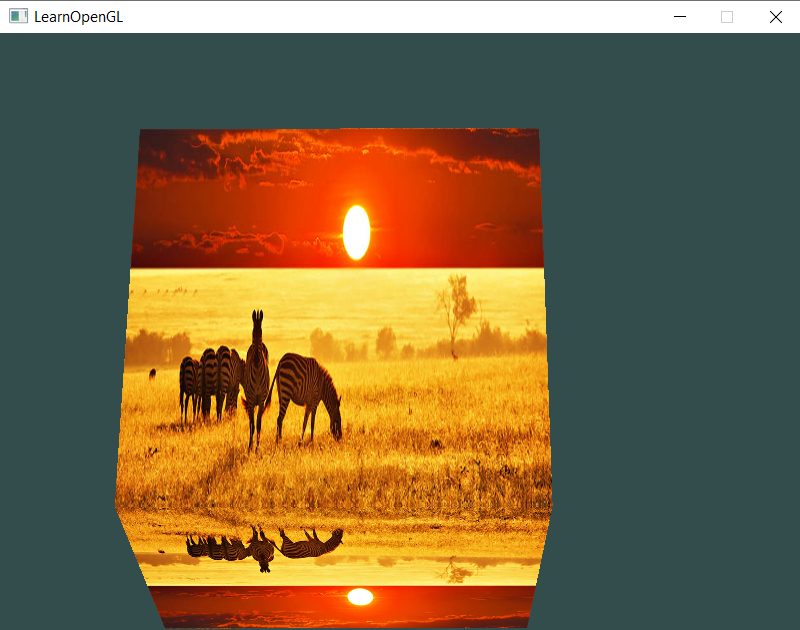
\includegraphics[width=.8\linewidth]{images/res_proj2.png}
      \caption{front}
      \label{fig:sfig1}
    \end{subfigure}%
    \begin{subfigure}{.5\textwidth}
      \centering
      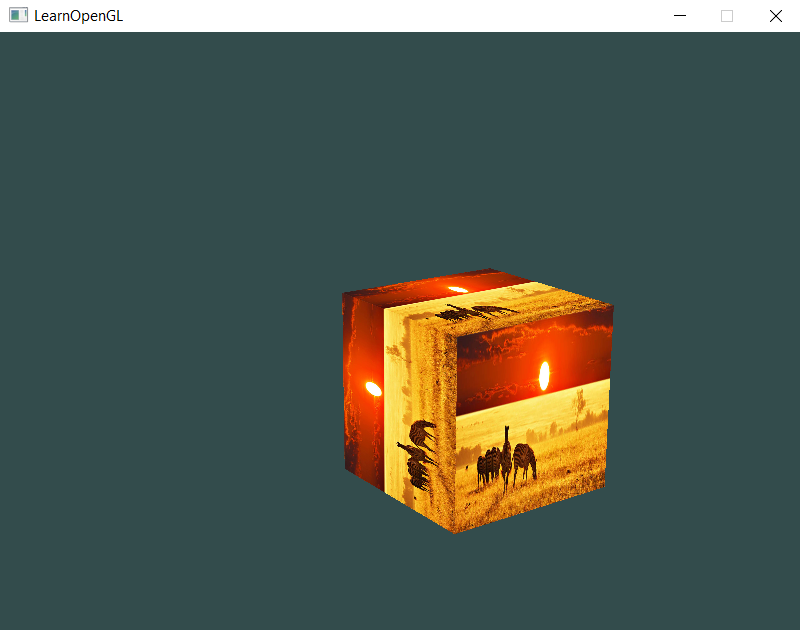
\includegraphics[width=.8\linewidth]{images/res_rotation.png}
      \caption{rotation}
      \label{fig:sfig2}
    \end{subfigure}
    \\
    \begin{subfigure}{.5\textwidth}
        \centering
        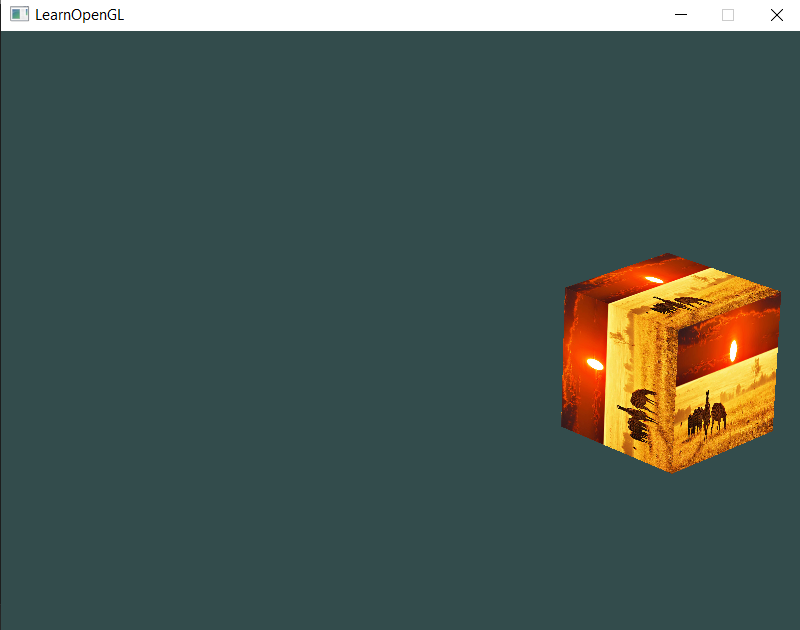
\includegraphics[width=.8\linewidth]{images/res_movement.png}
        \caption{movement}
        \label{fig:sfig2}
      \end{subfigure}
      \begin{subfigure}{.5\textwidth}
        \centering
        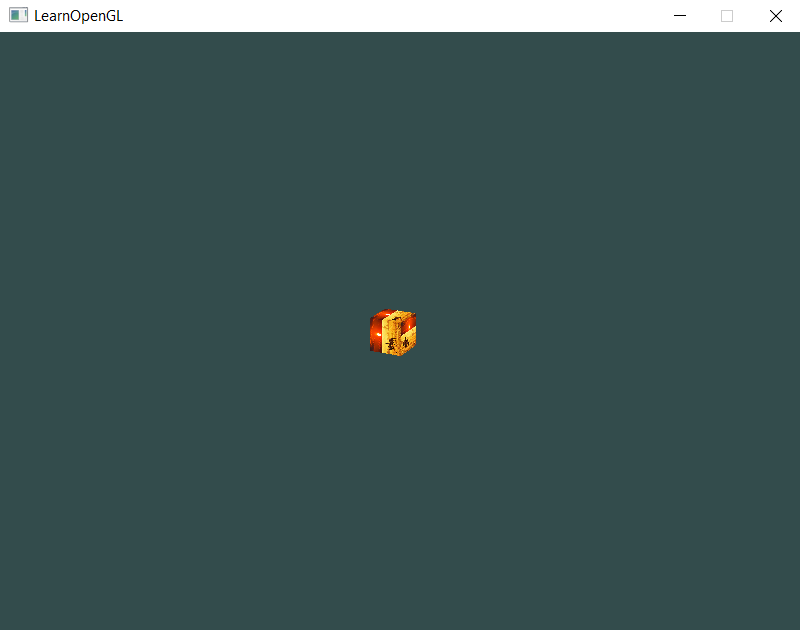
\includegraphics[width=.8\linewidth]{images/res_zoom.png}
        \caption{zoom}
        \label{fig:sfig2}
      \end{subfigure}
    \caption{Transformations}
    \label{fig:fig}
  \end{figure}

  \subsubsubsection{Emscripten компилятор}
  \noindent
  В коде синтаксис emscripten'a обрамляется \texttt{ifndef-else-endif}.
  Так же флаги, которые я использовал (их значения можно увидеть \href{https://emscripten.org/docs/tools_reference/emcc.html}{тут}):
  \begin{itemize}
    \item \texttt{FORCE\_FILESYSTEM=1}
    \item \texttt{USE\_WEBGL2=1}
    \item \texttt{USE\_GLFW=3}
    \item \texttt{FULL\_ES3=1}
    \item \texttt{ALLOW\_MEMORY\_GROWTH=1}
    \item \texttt{ASSERTIONS=1}
    \item \texttt{WASM=1}
  \end{itemize}
  \newpage
  Так же предоставляю результат, скомпилированный посредством emscripten:

  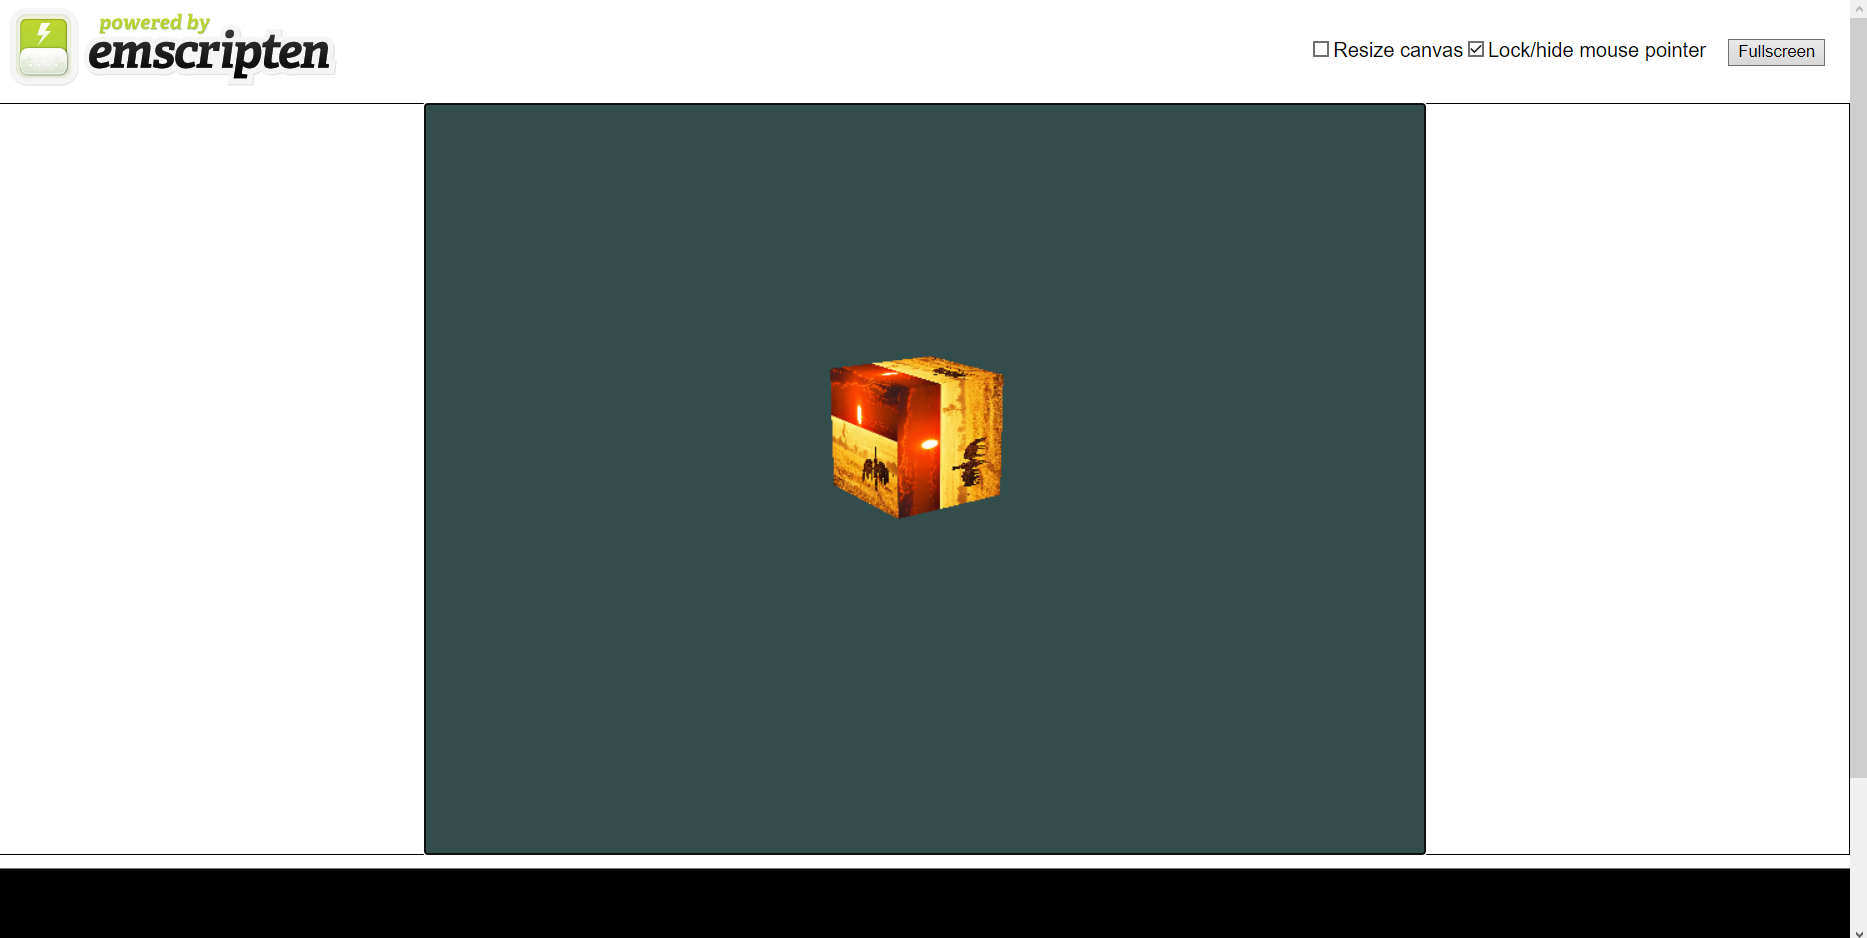
\includegraphics[width=\linewidth]{images/web_res.png}
  \subsection{Улучшения}
  Как я и говорил, мне осталось сделать свет и 3d object loader.
\end{document}